\section{Models} \label{model}
\begin{table}[t]
	\footnotesize
    \caption{Text generation models can be described across three dimensions: whether they suffer from exposure bias, 
whether they are trained in an end-to-end manner using back-propagation, 
and whether they are trained to predict one word ahead or the whole sequence.}
    \begin{tabular}{l || c | c | c |c}
      \multicolumn{1}{l||}{\em PROPERTY}  & 
      \multicolumn{1}{l|}{XENT} &
      \multicolumn{1}{l|}{DAD} & \multicolumn{1}{c|}{E2E} & \multicolumn{1}{c}{MIXER}\\
      \hline
      \hline
      {\em avoids exposure bias} & No & Yes & Yes & Yes \\
      \hline
      {\em end-to-end} & No & No & Yes & Yes \\
      \hline
      {\em sequence level} & No & No & No & Yes \\
    \end{tabular}
\label{tab:model_comparison}
\end{table}

The learning algorithms we describe in the following sections are agnostic to
the choice of the underlying model, as long as it is parametric. 
In this work, we focus on Recurrent Neural Networks (RNNs) as they are a popular choice for text generation. In particular, we use standard Elman RNNs~\citep{elman1990} and LSTMs~\citep{lstm}. For the sake of simplicity but without loss of generality, we discuss next Elman RNNs. This is a parametric 
model that at each time step $t$, takes as input a word $w_t \in \mathcal{W}$ as its input, together 
with an internal representation $\bh_t$. $\mathcal{W}$ is the the vocabulary of input words. 
This internal representation $\bh_t$ is a real-valued vector which encodes the history of 
words the model has seen so far. 
Optionally, the RNN can also take as input an  additional context vector $\bc_t$, which 
encodes the context to be used while generating the output. 
In our experiments $\bc_t$ is computed using an attentive decoder 
inspired by \cite{bahdanau-iclr2015} and \citet{rush-2015}, the details of which 
are given in Section ~\ref{sup-material:encoder} of the supplementary material. 
The RNN learns a recursive function to compute $\bh_t$ and 
outputs the distribution over the next word:
\begin{align}
    \bh_{t + 1} &= \phi_\theta(w_t, \bh_t, \bc_t),  \\
	w_{t+1} &\sim p_{\theta}(w |  w_t, \bh_{t+1}) =  p_{\theta}(w |  w_t, \phi_\theta(w_t, \bh_t, \bc_t)).
\end{align}
The parametric expression for $p_\theta$ and $\phi_\theta$ depends 
on the type of RNN. For Elman RNNs we have:
\begin{align}
\label{eq:elman-rnn}
    \bh_{t + 1} &= \sigma(M_i \bone(w_t) + M_h \bh_t + M_c \bc_t), \\
    \bo_{t+1} &= M_o \bh_{t+1}, \label{eq:softmax_input} \\
	w_{t+1} &\sim \mbox{softmax}(\bo_{t+1}),
    \label{eq:xent-distr}
\end{align}
where the parameters of the model $\theta$ are the set of matrices $\{M_o, M_i, M_h, M_c\}$ 
and also the additional parameters used to compute $\bc_t$. $\mbox{Softmax}(\bx)$ is a vector whose components are $e^{x_j} / \sum_k{e^{x_k}}$, and $\bone(i)$ is an indicator vector with only the $i$-th component set to $1$ and the rest to $0$. We assume the first word of the sequence is a special token indicating the beginning of a sequence, denoted by $w_1 = \varnothing$. All entries of the first hidden state $\bh_1$ are set to a constant value.

Next, we are going to introduce both baselines and the model we propose. As we describe these models, it is useful to keep in mind the key characteristics of a text generation system, as outlined in Table~\ref{tab:model_comparison}. There are three dimensions which are important when training a model for text generation: the exposure bias which can adversely affect generation at test time, the ability to fully back-propagate gradients (including with respect to the chosen inputs at each time step), and a loss operating at the sequence level. 
 We will start discussing models that do not possess any of these desirable features, and then move towards models that better satisfy our requirements. The last model we propose, dubbed MIXER, has all the desiderata.

\subsection{Word-Level Training}
We now review a collection of methodologies used for training text generation models which 
optimize the prediction of only one word ahead of time. 
We start with the simplest and the most popular method which optimizes the cross-entropy 
loss at every time step. We then discuss a recently proposed modification to it 
which explicitly uses the model predictions during training. 
We finish by proposing a simple yet novel baseline which uses its model prediction during 
training and also has the ability to back propagate the gradients through the entire sequence. 
While these extensions tend to make generation more robust, 
they still lack explicit supervision at the sequence level. 

\subsubsection{Cross Entropy Training (XENT)} \label{model-xent}
\begin{figure}[!t]
	   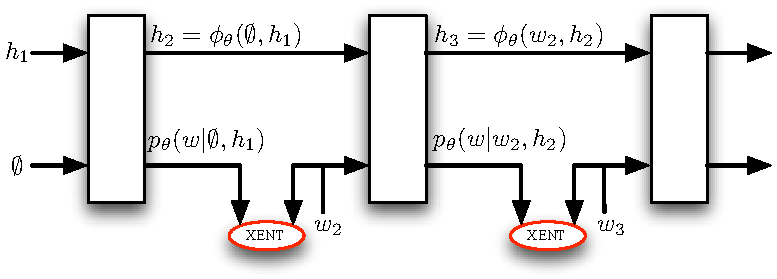
\includegraphics[width=0.65\linewidth]{xent_training.pdf}\\
	   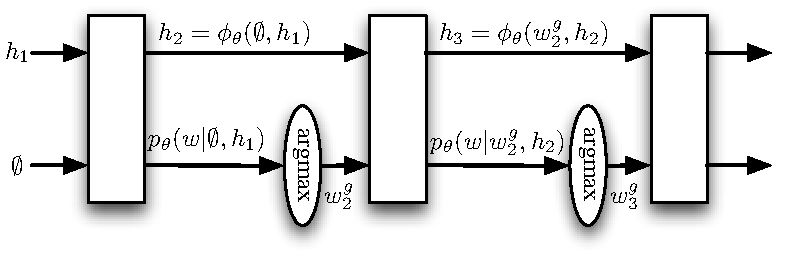
\includegraphics[width=0.65\linewidth]{xent_generation.pdf}
  \caption{RNN training using XENT (top), and how it is used at test time for generation (bottom). The RNN is unfolded for three time steps in this example. The red oval is a module computing a loss, while the rectangles represent the computation done by the RNN at one step. At the first step, all inputs are given. In the remaining steps, the input words are clamped to ground truth at training time, while they are clamped to model predictions (denoted by $w^g_t$) at test time. Predictions are produced by either taking the argmax or by sampling from the distribution over words. 
  % Additionally, the RNN can also take a context vector as input at each time step (not shown here).
  }
  \label{fig:xent}
\end{figure}
Cross-entropy loss (XENT) maximizes the probability of the observed sequence according to the model.
If the target sequence is $[w_1, w_2, \dots, w_T]$, then XENT training involves minimizing: 
\begin{align}
L =	- \log p(w_1, \ldots, w_T) = - \log \prod_{t=1}^T p(w_t | w_1, \ldots, w_{t-1}) = - \sum_{t=1}^T \log p(w_t | w_1, \ldots, w_{t-1}).  \label{eq:xenty}
\end{align}
When using an RNN, each term $p(w_t | w_1, \ldots, w_{t-1})$ is modeled as a parametric function as given in Equation~\eqref{eq:xent-distr}. This loss function trains the model to be good at greedily predicting the next word at each time step without considering the whole sequence. Training proceeds by truncated back-propagation through time~\citep{bptt} with gradient clipping~\citep{mikolov-2010}.

Once trained, one can use the model to generate an entire sequence as follows. Let $w^g_t$ denote the word generated by the model at the $t$-th time step. Then the next word  is generated by: 
\begin{align}
  \label{eq:greedy_gen}
  w^g_{t + 1} = \argmax_w p_{\theta}(w | w^g_t, \bh_{t+1}).
\end{align}
Notice that, the model is trained
to maximize $p_{\theta}(w | w_t, \bh_{t+1})$, where $w_t$ is the word in the ground truth sequence. However, during generation the model is used as  
$p_{\theta}(w | w^g_t, \bh_{t+1})$. In other words, during training the model is only exposed 
to the ground truth words. However, at test time the model has only
access to its own predictions, which may not be correct. As a result, during generation the model can potentially deviate quite far from the actual sequence to be generated. Figure~\ref{fig:xent} illustrates this discrepancy. 

The generation described by Eq.~\eqref{eq:greedy_gen} is
a greedy left-to-right process which does not necessarily produce
the most likely sequence according to the model, because:
\begin{align*}
    \prod_{t=1}^T ~\max_{w_{t+1}}~p_{\theta}(w_{t+1} | w^g_t, \bh_{t+1}) \leq
    \max_{w_1, \dots, w_T}~\prod_{t=1}^Tp_{\theta}(w_{t+1} | w^g_t, \bh_{t+1})
\end{align*}
The most likely sequence $[w_1, w_2, \dots, w_T]$ might contain a word  $w_t$ which is sub-optimal at an intermediate time-step $t$. This phenomena is commonly known as a {\it search error}. 
One popular way to reduce the effect of search error is to pursue not only one but $k$ next word 
candidates at each point. While still approximate, this strategy can recover 
higher scoring sequences that are often also better in terms of our final evaluation metric.
This process is commonly know as {\it Beam Search}. The downside of using beam search is that it significantly slows down 
the generation process. The time complexity 
grows linearly in the number of beams $k$, because we need to perform 
$k$ forward passes for our network, which is the most time intensive operation. 
The details of the 
Beam Search algorithm are described in Section~\ref{sup-material:beam_search}.


%\noindent{\bf Beam Search}  
%Equation~\ref{eq:greedy_gen} always chooses the highest scoring next word candidate
%at each time step. At test time we can reduce the effect of search error 
%by pursuing not only one but $k$ next word candidates at each point, which 
%is commonly known as {\it beam search}.
%While still approximate, this strategy can recover higher scoring sequences 
%that are often also better in terms of our final evaluation metric.
%The algorithm maintains the $k$ highest scoring partial
%sequences, where $k$ is a hyper-parameter.
%Setting $k=1$ reduces the algorithm to a greedy left-to-right search 
%(Eq.~\eqref{eq:greedy_gen}). 
%The downside of such an exploration of multiple paths is that it significantly slows down the generation process. The time complexity 
%grows linearly in $k$ because we need to perform $k$ forward passes for our network which is the most time intensive operation. 
%As a result, beam search generation is $k$ times slower than greedy search (Eq.~\eqref{eq:greedy_gen}). Pseudo-code of beam search is shown in Algorithm~\ref{alg:beam} of our Supplementary Material.

\subsubsection{Data As Demonstrator (DAD)} \label{model-dad}
\begin{figure}[!t]
\begin{center}
% \vspace{-.5cm}
 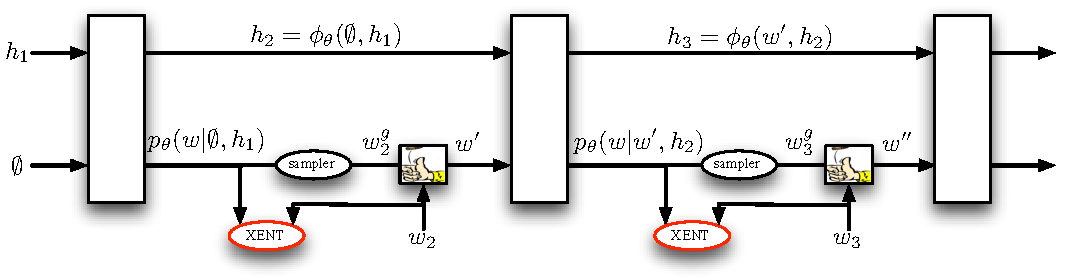
\includegraphics[width=0.7\linewidth]{dad.pdf}
%  \vspace{-.5cm}
\end{center}
\caption{Illustration of DAD~\citep{sbengio-nips2015,
    dad}. Training
  proceeds similar to XENT, except that at each time step we choose with
  a certain probability whether to take the previous model prediction or
  the ground truth word. Notice how a) gradients are not
  back-propagated through the eventual model predictions $w^g_t$, and
  b) the XENT loss always uses as target the next word in the reference
  sequence, even when the input is $w^g_t$.}
\label{fig:dad}
\end{figure}
Conventional training with XENT suffers from exposure bias since  
training uses ground truth words as opposed to model predictions.
DAD, proposed in~\citep{dad} and also used in~\citep{sbengio-nips2015} for sequence generation, addresses this issue by mixing the ground truth training data with model predictions.
At each time step and with a certain probability, DAD takes as input either the prediction from the model at the previous time step or the ground truth data. \citet{sbengio-nips2015} proposed  different 
annealing schedules for the probability of choosing the ground truth word. The annealing schedules are such that at the beginning, the algorithm always chooses the ground truth words. However, as the training progresses the model predictions are selected more often. 
This has the effect of making the model somewhat more aware of how it will be used at test time. Figure~\ref{fig:dad} illustrates the algorithm. 

A major limitation of DAD is that at every time step the target labels are always selected from the ground truth data,  regardless of how the input was chosen. As a result, the targets may not be aligned with the generated sequence, forcing the model to predict a potentially incorrect sequence. 
For instance, if the ground truth sequence is ``I took a long
walk" and the model has so far predicted ``I took a walk", DAD will force the model to predict the word ``walk" a second time. 
Finally, gradients are not back-propagated through the samples drawn by the model and the XENT loss is still at the word level. 
It is not well understood how these problems affect generation.

\subsubsection{End-to-End BackProp (E2E)} 
\label{model-e2e}
%In our quest to bridge the gap between the way the text generation models are trained and the way they are used, we also experimented with a novel modification to the standard training of RNNs. 
The novel E2E algorithm is perhaps the most natural and na\"{\i}ve approach approximating sequence level training, which can also be interpreted as a computationally efficient approximation to beam search. 
The key idea is that at time step $t + 1$ we propagate as input the top $k$ words predicted at the previous time step instead of the ground truth word. 
Specifically, we take the output distribution over words from the previous time step $t$, and pass it through a $k$-max layer. 
This layer zeros all but the $k$ largest values and re-normalizes 
them to sum to one. We thus have: 
%The re-normalized distribution is used as input at the current time step $t+1$:
\begin{equation}
\{i_{t+1,j}, v_{t+1,j}\}_{j=1, \dots, k} = \mbox{k-max } p_\theta(w_{t+1} |  w_t, h_t), \label{eq:e2e}
\end{equation}
where $i_{t+1,j}$ are indexes of the words with $k$ largest probabilities and $v_{t+1,j}$ are their corresponding scores. 
At the time step $t+1$, we take the $k$ largest scoring previous words as input whose 
contributions is weighted by their scores $v$'s. 
Smoothing the input this way makes the whole process 
differentiable and trainable using standard back-propagation.
%of the error using the cross-entropy loss of Equation~\ref{eq:xenty}. 
Compared to beam search, this can be interpreted as fusing the $k$ possible next 
hypotheses together into a single path, as illustrated in Figure~\ref{fig:e2e}. 
In practice we also employ a schedule, whereby we use only the ground truth words 
at the beginning and gradually let the model use its own top-$k$ predictions as training proceeds. 
%After a few epochs, we use top-$k$ predictions for the last $\Delta$ steps of the sequence. 
%Afterwards, the RNN uses its own predictions for the last $2 \Delta$ steps, on so on so forth. 

While this algorithm is a simple way to expose the model to its own predictions, the loss function optimized is still XENT at each time step. 
There is no explicit supervision at the sequence level while training the model. 
\begin{figure}[!t]
\begin{center}
% \vspace{-.5cm}
 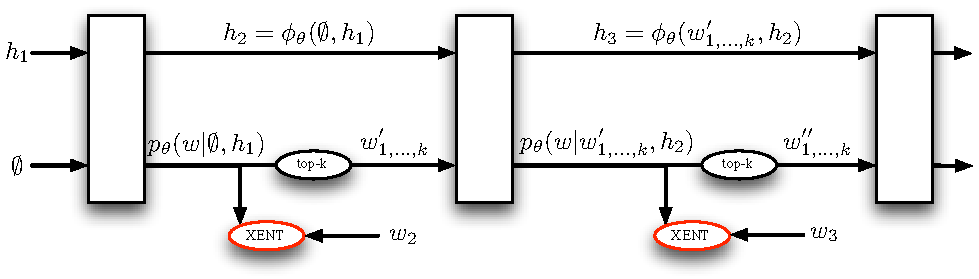
\includegraphics[width=0.7\linewidth]{e2e.pdf}
% \vspace{-.5cm}
\end{center}
\caption{Illustration of the End-to-End BackProp method. The first 
  steps of the unrolled sequence (here just the first step) are exactly the same
  as in a regular RNN trained with cross-entropy. However, in the remaining
  steps the input to each module is a sparse
  vector whose non-zero entries are the $k$ largest probabilities
  of the distribution predicted at the previous time step. Errors are
  back-propagated through these inputs as well.}
\label{fig:e2e}
\end{figure}

\subsection{Sequence Level Training}
We now introduce a novel algorithm for sequence level training, which we call Mixed Incremental Cross-Entropy Reinforce (MIXER). The proposed method avoids the exposure bias problem, 
and also directly optimizes for the final evaluation metric. 
Since MIXER is an extension of the REINFORCE algorithm, we first describe REINFORCE 
from the perspective of sequence generation. 

\subsubsection{REINFORCE} \label{model-reinforce}
In order to apply the REINFORCE algorithm~\citep{reinforce, zaremba-arxiv2015} to the problem of sequence generation we cast our problem in the reinforcement learning (RL) framework~\citep{sutton-rl}. Our generative model (the RNN) can be viewed as an {\em agent}, which interacts with the external environment (the words and the context vector it sees as input at every time step). The parameters of this agent defines a {\em policy}, whose execution results in the agent picking an {\em action}. In the sequence generation setting, an action refers to predicting the next word in the sequence at each time step. 
After taking an action the agent updates its internal state (the hidden units of RNN). Once the agent has reached the end of a sequence, it observes a {\em reward}. We can choose any reward function. Here, we use BLEU~\citep{bleu} and ROUGE-2~\citep{rouge} since these are the metrics we use at test time. BLEU is essentially a geometric mean over n-gram precision scores  as well as a brevity penalty~\citep{liang2006}; in this work, we consider up to $4$-grams. ROUGE-2 is instead recall over bi-grams. 
Like in {\em imitation learning}, we have a training set of optimal sequences of actions. 
During training we choose actions according to the current policy and only observe a reward at the end of the sequence (or after maximum sequence length), by comparing the sequence of actions from the current policy against the optimal action sequence.
The goal of training is to find the parameters of the agent that maximize the expected reward.
We define our loss as the negative expected reward:
\begin{align}
L_{\theta} = - \sum_{w^g_1, \dots, w^g_T} p_\theta(w^g_1, \dots,
w^g_T) r(w^g_1, \dots, w^g_T) = -\mathbb{E}_{[w_1^g, \dots w^g_T] \sim p_\theta} r(w^g_1, \dots, w^g_T), \label{eq:reinforce-loss}
\end{align}
where $w^g_n$ is the word chosen by our model at the $n$-th time step, and $r$ is the reward associated with the generated sequence. 
In practice, we approximate this expectation with a single sample
from the distribution of actions implemented by the RNN (right hand side of the equation above and Figure~\ref{fig:plan} of Supplementary Material). 
We refer the reader to prior work~\citep{zaremba-arxiv2015,reinforce} for the full derivation of the gradients. Here, we directly report the partial derivatives and their interpretation. The derivatives w.r.t. parameters are:
\begin{equation}
\frac{\partial L_{\theta}}{\partial \theta} = \sum_t \frac{\partial L_{\theta}}{\partial \bo_t}
\frac{\partial \bo_t}{\partial \theta} \label{eq:reinf-deriv1}
\end{equation}
where $\bo_t$ is the input to the softmax. 
The gradient of the loss $L_{\theta}$ with respect to $\bo_t$ is given by:
\begin{equation}
\frac{\partial L_{\theta}}{\partial \bo_t} = \left( r(w^g_1, \dots, w^g_T) - \bar{r}_{t+1} \right) \left( p_\theta(w_{t+1} | w^g_{t}, \bh_{t+1}, \bc_t) - \bone(w^g_{t+1}) \right),
 \label{eq:reinf-deriv2}
\end{equation}
where $\bar{r}_{t+1}$ is the average reward at time $t + 1$. 

The interpretation of this weight update rule is straightforward. While
Equation~\ref{eq:reinf-deriv1} is standard back-propagation (a.k.a. chain
rule), Equation~\ref{eq:reinf-deriv2} is almost exactly the same as the gradient of a multi-class logistic regression classifier. In logistic regression, the gradient is the difference between the prediction and the actual 1-of-N representation of the target word:
\begin{equation*}
\frac{\partial L^{\mbox{\small XENT}}_{\theta}}{\partial \bo_t} 
 =  p_\theta(w_{t+1} | w_{t}, \bh_{t+1}, \bc_t) - \bone(w_{t+1})
\end{equation*}
Therefore, Equation~\ref{eq:reinf-deriv2} says that the chosen word $w^g_{t+1}$
acts like a surrogate target for our output distribution,
$p_\theta(w_{t+1}|w^g_{t}, \bh_{t+1}, \bc_t)$ at time $t$. REINFORCE first establishes a baseline $\bar{r}_{t+1}$,
and then either encourages a word choice $w^g_{t+1}$ if $r > \bar{r}_{t+1}$, 
or discourages it if $r < \bar{r}_{t+1}$. The actual derivation suggests that the choice of this average reward $\bar{r}_t$ is useful to decrease the variance of the gradient estimator since in Equation~\ref{eq:reinforce-loss} we use a single sample from the distribution of actions. 

In our implementation, the baseline $\bar{r}_t$ is estimated by a linear regressor which takes as input the hidden states $\bh_t$ of the RNN. The regressor is an unbiased estimator of future rewards since it only uses past information. The parameters of the regressor are
trained by minimizing the mean squared loss: $||\bar{r}_t - r||^2$.
In order to prevent feedback loops, we do not backpropagate this error through
the recurrent network~\citep{zaremba-arxiv2015}. 

REINFORCE is an elegant algorithm to train at the sequence level using {\em any} user-defined reward. In this work, we use BLEU and ROUGE-2 as reward, however one could just as easily use any other metric.
When presented as is, one major drawback associated with the algorithm is that it assumes a random
policy to start with. This assumption can make the learning for large action spaces very challenging.
Unfortunately, text generation is such a setting where the cardinality of the action set is in the order of $10^4$ (the number of words in the vocabulary). 
This leads to a very high branching factor where it is extremely hard for a random policy to improve in any reasonable amount of time. 
In the next section we describe the MIXER algorithm which addresses these issues, better targeting
text generation applications.

\subsubsection{Mixed Incremental Cross-Entropy Reinforce (MIXER)} \label{model-mixer}
The MIXER algorithm borrows ideas both from DAGGER~\citep{dagger} and 
DAD~\citep{dad, sbengio-nips2015} and modifies the REINFORCE appropriately. 
The first key idea is to change the initial policy of REINFORCE to make sure
the model can effectively deal with the large action space of text generation.
Instead of starting from a poor random policy and training the model to converge 
towards the optimal policy, we do the exact opposite. We start from the optimal 
policy and then slowly deviate from it to let the model explore and make use 
of its own predictions.
% Instead of trying to make
% the random policy converge to the optimal policy, we
% do the opposite: we start with the optimal policy and we slowly
% deviate from it to let the model explore and make use of its own
% predicitons. 
We first train the RNN with the cross-entropy loss for
$N^{\mbox{\small{XENT}}}$ epochs using the ground truth sequences.
This ensures that we start off with a much better policy than random 
because now the model can focus on a good part of the search space.
This can be better understood by comparing the perplexity of a language model 
that is randomly initialized versus one that is trained. Perplexity is a measure of uncertainty of the prediction and, roughly speaking, it corresponds to the average number of words the model is `hesitating' about when making a prediction. A good language model trained on one of our data sets has perplexity of $50$, whereas a random model is likely to have
perplexity close to the size of the vocabulary, which is about $10,000$.
% This ensures that we start off with a good policy and drastically reduce the search space, since a good language model on one of our datasets has perplexity of about 50 as opposed to the size of the dictionary.\footnote{Perplexity can be thought of
% as the effective number of words in the dictionary, as it is related
% to the average number of words the model is confused about when it makes a prediction.}.
\begin{figure}[!t]
\begin{center}
% \vspace{-.5cm}
 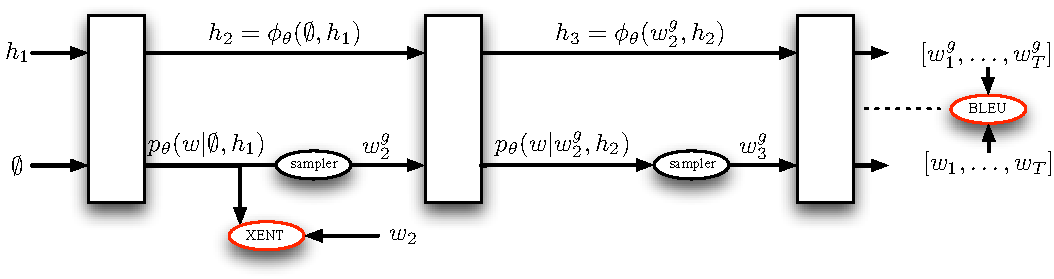
\includegraphics[width=0.75\linewidth]{mixer.pdf}
% \vspace{-.5cm}
\end{center}
\caption{Illustration of MIXER. In the first $s$ unrolling steps (here $s=1$),
  the network resembles a standard RNN trained by XENT. In the
  remaining steps, the input to each module is a sample from the
  distribution over words produced at the previous time step. Once the
  end of sentence is reached (or the maximum sequence length), a
  reward is computed, e.g., BLEU. REINFORCE is then
  used to back-propagate the gradients through the sequence of
  samplers. We employ an annealing schedule on $s$, starting with 
  $s$ equal to the maximum sequence length $T$ and finishing with $s = 1$.
 }
\label{fig:mixer}
\end{figure}

The second idea is to introduce model predictions during training 
with an annealing schedule in order to gradually teach the model to produce stable sequences. 
Let $T$ be the length of the sequence.
After the initial $N^{\mbox{\small{XENT}}}$ epochs, we continue training the 
model for $N^{\mbox{\small{XE+R}}}$ epochs, such that, for every sequence 
we use the XENT loss for the first ($T - \Delta$) steps, and the REINFORCE algorithm 
for the remaining $\Delta$ steps.
%After the initial $N^{\mbox{\small{XENT}}}$ epochs, we perform the next
%$N^{\mbox{\small{XE+R}}}$ epochs applying XENT loss to the first ($T - \Delta$)
%steps, and REINFORCE to the remaining $\Delta$ steps. 
In our experiments $\Delta$ is typically set to two or three. 
Next we anneal the number of steps for which we use the XENT loss for every sequence to  
($T - 2 \Delta$) and repeat the training for another $N^{\mbox{\small{XE+R}}}$ epochs. 
We repeat this process until only REINFORCE is used to train the whole sequence.
See Algorithm~\ref{alg:mixer} for the pseudo-code. 

%Afterwards, we apply XENT loss to the first 
%($T - 2 \Delta$) steps, and reinforce to the remaining $2 \Delta$ steps,
%and so forth (see alg.~\ref{alg:mixer}).

We call this algorithm Mixed Incremental Cross-Entropy Reinforce (MIXER)
because we combine both XENT and REINFORCE, and we use incremental 
learning (a.k.a. curriculum learning). 
The overall algorithm is illustrated in Figure~\ref{fig:mixer}. 
By the end of training, the model can make effective use of its own 
predictions in-line with its use at test time.

\begin{algorithm}[t]
% \vspace{-1cm}
\footnotesize
 \KwData{a set of sequences with their corresponding context.}
 \KwResult{RNN optimized for generation.}
 Initialize RNN at random and set $N^{\mbox{\small{XENT}}}$, $N^{\mbox{\small{XE+R}}}$
 and $\Delta$\; 
 \For{$s$ = $T$, $1$, $-\Delta$}{
   \eIf{ $s$ == $T$ }{
     train RNN for $N^{\mbox{\small{XENT}}}$ epochs using XENT only\;
     }{
     train RNN for $N^{\mbox{\small{XE+R}}}$ epochs. Use XENT loss in the
     first $s$ steps, and REINFORCE (sampling from the model) in the remaining $T - s$ steps\;
   }
 }
%  \vspace{-.25cm}
 \caption{MIXER pseudo-code.}
 \label{alg:mixer}
\end{algorithm}
